\section{Testing Environment}

\begin{figure}[H]
\centerline{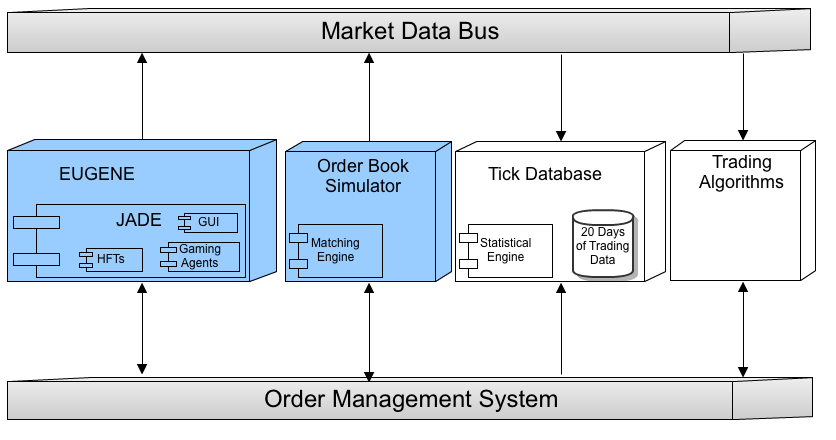
\includegraphics[scale=0.5]{architectural-description/automated-trading-testing-environment.png}}
\caption{Automated Trading Algorithm Testing Environment}
\label{fig:automated-trading-algorithm-testing-environment}
\end{figure}

Trading Algorithms respond to messages received from the Stock Exchange (via the Market Data Bus) and send orders to the Stock Exchange (via the Order Management System). They expect the orders to have some influence on the situation on the Stock Exchange. 

Therefore, in order to setup a testing environment for Trading Algorithms, two systems need to be put in place in order to simulate the Trading System.

\subsection{Order Book Simulator}
Order Matching Engine which can accept orders in to Continuous Auction Trading and match Bid/Sell orders. The simulator should be programmable to handle any number of exchanges and stocks. Such an engine is already available for use and will not be the subject of this project.

\subsection{Market Behaviour Simulator}
Market Behaviour Simulator that can realistically simulate a broad range of market behaviours (e.g. rising and falling, flash crash, gaming). This project will propose a design of such a Market Simulator using an Agent-Based Approach.
